\section{Mathematische Modelle \skript{27}}
\subsection{Deskriptive Modelle und Optimierungsmodelle \skript{27}}
  \begin{tabular}{|p{3.7cm}|p{7cm}|p{7cm}|}
    \hline
    & \textbf{Deskriptive Modelle}
    & \textbf{Optimierungsmodelle} \\
    \hline
    \hline
    Antworten auf\ldots
      & ``What if?''
      & ``What's best?'' \\
    \hline
    Mengen ($I$)
      & \multicolumn{2}{l|}{Typen von Objekten (z.B. Städte $I = \{1,2,\ldots,n\}$)} \\
    \hline
    Parameter ($p_i$)
      & \multicolumn{2}{p{14cm}|}{Vorgebene Grössen des Modells (z.B. aktueller Fahrzeugbestand in Filiale $i$, Distanz zwischen Filiale $i$ und $j$)} \\
    \hline
    Variablen ($x_{ij}$)
      & \multicolumn{2}{l|}{Veränderbare Modellgrösse (z.B. Anz. transferierte Fahrzeuge von Filiale $i$ nach $j$)} \\
    \hline
    Konsequenzen ($k_{i}, k_i^{out}$)
      & Output des deskriptiven Modells (z.B. gesamte Fahrdistanz), $k_0 = f_0(x,p)$ 
      & -\\
    \hline
    Zielfunktion $\min$ oder $\max$
      & - 
      & Zu maximierende oder minimierende Konsequenz\\
    \hline
    Restriktionen / Constraints ($k_{i}, k_i^{out}$)
      & - 
      & Bedingungen auf den Konsequenzen (Ungleichungen, selten Gleichungen) ACHTUNG: 'Idiotische' Bedingungen nicht vergessen: Keine negativen Mengen produzieren, etc.\\
    \hline
  \end{tabular}
  
  \subsubsection{Beispiel für Modellierung (Klinkert, Übung 4, Aufgabe 5)}
  Aus den Edelmetallen $I$ sollen die Legierungen $J$ gemischt werden. Der Erlös soll maximiert werden.\\
  Mengen:\\
  \begin{tabular}{lll}
    $I$ & Menge der Edelmetalle, &$I = \{1, \ldots, m\}$\\
    $J$ & Menge der Legierungen, &$J = \{1, \ldots, n\}$
  \end{tabular}\\
  Parameter:\\
  \begin{tabular}{lll}
    $a_{ij}$ & Menge von Edelmetall $i$ pro Menge Legierung $j$ & $i \in I, j \in J$\\
    $b_i$    & Verfügbare Menge von Edelmetall $i$              & $i \in I$\\
    $c_i$    & Erlös pro Menge Legierung $j$                    & $j \in J$\\
  \end{tabular}\\
  Variablen:\\
  \begin{tabular}{lll}
    $x_j$ & Produktionsmenge von Legierung $j$ & $j \in J$\\
  \end{tabular}\\
  Zielfunktion:\\
  \begin{tabular}{l}
    max $\sum_{j \in J}c_j x_j$\\
  \end{tabular}\\
  Restriktionen:\\
  \begin{tabular}{lll}
    $\sum_{j \in J}a_{ij}x_j \le b_i$ & $i \in I$ & (nicht mehr Legierung produzieren als Edelmetall vorhanden)\\
    $x_j \ge 0$                       & $j \in J$ & (nicht negative Mengen Legierungen produzieren)
  \end{tabular}\\




\subsection{Allgemeines Optimierungsproblem \skript{31}}
  In Form von Ungleichungen und Gleichungen werden mögliche Lösungsmengen (\em solution spaces \em) definiert. Dort soll eine Zielfunktion $f$ optimiert (maximiert oder minimiert) werden. Die Fragestellung lautet: "`What's best?"' (preskriptive Modelle).
  
  \begin{center}
    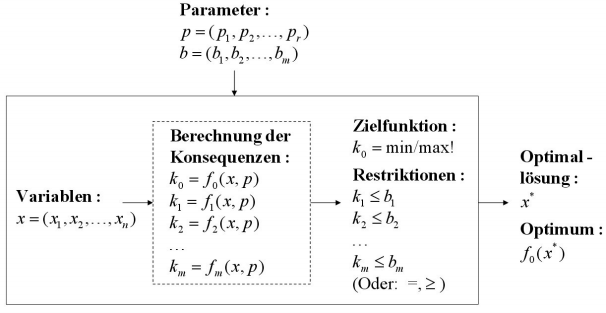
\includegraphics[width=10cm]{./Content/OptMathModels/OptimiziationModel}
  \end{center}
  
  \begin{tabularx}{\textwidth}{p{7cm} X}
  \hline
    \textbf{Problemformulierung} & \\
  \hline
    Allgemeines Optimierungsproblem
      & $\Pi: \max\{f(x) : x \in S\}$ wobei $S \subseteq \mathbb{R}^n$\\
    Entscheidungsvariablen/Variablen (\em decision variables/variables\em)
      & Vektor $x = (x_1, ..., x_n) \in \mathbb{R}^n$\\
    Lösungsmenge/Lösungsraum (\em solution space, feasible region\em)
      & $S$ von $\Pi$\\
    Zielfunktion
      & $f: S \rightarrow \mathbb{R}$\\
    Zulässigkeit (\em feasibility\em)
      & Lösungsraum darf nicht leer sein ($S \neq 0$)\\
    Beschränktheit (\em bounded\em)
      & $f(x) \leq \omega,\, \omega \in \mathbb{R}$ für alle $x \in S$\\
    Abgeschlossenheit (\em closed\em)
      & Zusätzlich zu Zulässigkeit und Beschränktheit: $x^* \in S$ (Optimallösung existiert)\\
  \hline
    \textbf{Definition des Lösungsraums} & \\
  \hline
    Funktionale Restriktionen (\em functional constraints\em)
      & $p\geq 0$ Ungleichungen der Form $g_i(x) \leq 0$, \newline
        $q \geq 0$ Ungleichungen der Form $h_j(x) = 0$.\newline
        $g_i(x), h_j(x)$ sind lineare Funktionen!\\
    Nicht-funktionale Restriktionen 
      & Definition des Lösungsraums $S$ durch "`nicht-funktionale"' Restriktionen, z.B. logische Prädikate (z.B. $S=\{x \in \mathbb{Z}^n: x \text{ ist eine Permutation der Zahlen } 1,...,n \}$) \\
  \hline
    \textbf{Maximierungs-/Minimierungsprobleme} & Beides möglich, Umwandlung siehe \ref{sec:linprog_umwandlungen}\\
  \hline
    Extremwert-Theorem von Weierstrasse
      & Wenn $S \subseteq \mathbb{R}^n$ eine nichtleere, begrenzte, abgeschlossene Menge und $f: S \rightarrow \mathbb{R}$ eine stetige Funktion ist, existiert ein $x^* \in S$ mit $f(x^*) \geq f(x)$
       für alle $x \in S$, d.h. das Optimierungsproblem hat eine Optimallösung.\\
  \hline
    \textbf{Nachbarschaft (\em Neighbourhood\em)} & Beliebige Menge Punkte "`in der Nähe"' des aktuellen Punktes $x$\\
  \hline
    Euklidische Nachbarschaft
      & $N_\epsilon(x) = \{ y \in \mathbb{R}^n: ||y-x|| \leq \epsilon \}$ mit $\epsilon > 0$, $||x|| = \sqrt{x^2} = \sqrt{x_1^2 + ... + x_n^n}$ (in $\mathbb{R}^2$ eine Kreis, $\mathbb{R}^3$ eine Kugel, etc.)\\
    Andere Nachbarschaften
      & Es sind auch andere Nachbarschaftsdefinitionen möglich (ohne Bsp.)\\
  \hline
    \textbf{Diverses} &\\
  \hline
      Globale Optimallösung
      & $x^*$ ist eine globale Optimallösung wenn $f(x^*) \geq f(x)$ für alle $x \in S$.\\
    Lokale Optima
      & $x^*$ ist eine lokale Optimallösung (bzgl. Nachbarschaft $N_\epsilon$) wenn $f(x^*) \geq f(x)$ für alle $x \in N_\epsilon(x^*) \cap S$\\
    Niveaumengen (Höhenlinien, \em level sets\em)
      & Orthogonale Linien zu den linearen Funktionen (Geraden)\\      
  \end{tabularx}
  

\subsection{Konvexe Optimierung \skript{40}}
  \begin{tabularx}{\textwidth}{p{6cm} X}
  \hline
    \textbf{Definitionen} & \\
  \hline
    $\lambda$
      & $\lambda \in \mathbb{R}$ mit $0 \leq \lambda \leq 1$\\
    Konvexkombination zweier Vektoren
      & $x^1, x^2 \in \mathbb{R}^n$:  $x = \lambda x^1 + (1-\lambda) x^2$ \\
    Konvexe Funktion
      & $f(\lambda x^1 + (1-\lambda)x^2) \leq \lambda f(x^1) + (1-\lambda)f(x^2)$ für alle $x^1, x^2 \in S$, $S$ konvex \newline
      Deutsch: Lineare Interpolation zwischen $x^1$ und $x^2$ ist kleiner gleich als Funktion\\
    Konkave Funktion
      & $f(\lambda x^1 + (1-\lambda)x^2) \geq \lambda f(x^1) + (1-\lambda)f(x^2)$ für alle $x^1, x^2 \in S$, $S$ konvex \newline
      Deutsch: Lineare Interpolation zwischen $x^1$ und $x^2$ ist grösser gleich als Funktion\\
    Lineare Funktion
      & Eine lineare Funktion ist sowohl konvex als auch konkav in $S$.\\
    Konvexe Menge
      & $\lambda x^1 + (1-\lambda)x^2 \in S$ für Vektoren $x^1,x^2 \in S \subseteq \mathbb{R}^n, \lambda \in \mathbb{R}, 0 \leq \lambda \leq 1$.\newline
      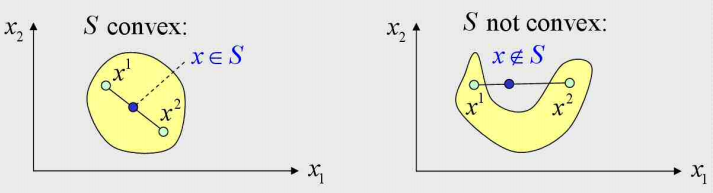
\includegraphics[width=7cm]{./Content/OptMathModels/ConvexSet} \\
    Konvexes Optimierungsproblem
      & Ein konvexes Optimierungsproblem ist \em entweder \em die Maximierung einer konkaven Funktion $f$ über einer konvexen Menge $S$ \em oder \em die Minimierung einer konvexen Funktion $f$ über einer konvexen Menge $S$.\\
  \hline  
    \textbf{Eigenschaften} & \\
  \hline
    Globales Optimum
      & In einem konvexen Optimierungsproblem ist jedes lokales Optimum ein globales Optimum! \\
    Optimum auf Rand
      & $S \subseteq \mathbb{R}^n$ sei eine konvexe, abgeschlossene, begrenzte Menge. Bei einem Optimierungsproblem der Form $\max\{ f(x) : x \in S \}$ (bzw. $\min\{ f(x) : x \in S \}$) mit $f$ konvex (bzw. konkav) in $S$ liegt jede lokale Optimallösung auf dem Rand. \newline 
      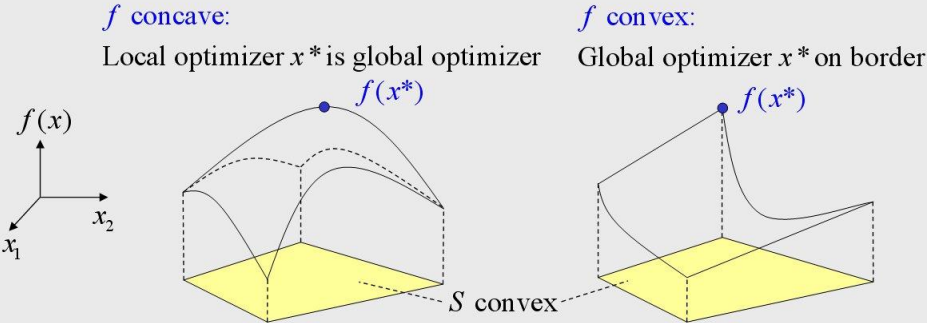
\includegraphics[width=8cm]{./Content/OptMathModels/ConvexBorderSolution}
      \\
    Lineare Funktion
      & Für den Fall einer linearen Funktion $f$ über einer konvexen, begrenzten, abgeschlossenen Menge $S$ gilt, dass jede lokale Optimallösung global optimal ist und sich am Rand von $S$ befindet!\\
  \end{tabularx}
  
  \todo{Mengenlehre reinnehmen}
\subsection{Typen von Optimierungsmodellen und -methoden \skript{46}}

